\documentclass[10pt]{article}

\usepackage[utf8x]{inputenc}
\usepackage{latexsym, amsmath, amsfonts, amsthm, amssymb}
\usepackage[document]{ragged2e}

\usepackage[usenames, dvipsnames]{color}
\usepackage{gensymb}
\usepackage{graphicx}

\usepackage{color}
\usepackage{listings}
\usepackage{setspace}

\definecolor{Code}{rgb}{0,0,0}
\definecolor{Decorators}{rgb}{0.5,0.5,0.5}
\definecolor{Numbers}{rgb}{0.5,0,0}
\definecolor{MatchingBrackets}{rgb}{0.25,0.5,0.5}
\definecolor{Keywords}{rgb}{0,0,1}
\definecolor{self}{rgb}{0,0,0}
\definecolor{Strings}{rgb}{0,0.63,0}
\definecolor{Comments}{rgb}{1,0,0}
\definecolor{Backquotes}{rgb}{0,0,0}
\definecolor{Classname}{rgb}{0,0,0}
\definecolor{FunctionName}{rgb}{0,0,0}
\definecolor{Operators}{rgb}{0,0,0}
\definecolor{Background}{rgb}{0.98,0.98,0.98}

\lstnewenvironment{python}[1][]{
\lstset{
numbers=left,
numberstyle=\footnotesize,
numbersep=1em,
xleftmargin=1em,
framextopmargin=2em,
framexbottommargin=2em,
showspaces=false,
showtabs=false,
showstringspaces=false,
frame=l,
tabsize=2,
% Basic
basicstyle=\ttfamily\small\setstretch{1},
backgroundcolor=\color{Background},
language=Python,
% Comments
commentstyle=\color{Comments}\slshape,
% Strings
stringstyle=\color{Strings},
morecomment=[s][\color{Strings}]{"""}{"""},
morecomment=[s][\color{Strings}]{'''}{'''},
% keywords
morekeywords={import,from,class,def,for,while,if,is,in,elif,else,not,and,or,print,break,continue,return,True,False,None,access,as,,del,except,exec,finally,global,import,lambda,pass,print,raise,try,assert},
keywordstyle={\color{Keywords}\bfseries},
% additional keywords
morekeywords={[2]@invariant},
keywordstyle={[2]\color{Decorators}\slshape},
emph={self},
emphstyle={\color{self}\slshape},
%
}}{}


\begin{document}
\title{CC Neurosciences Computationnelles}
\author{\texttt{Rodriguez Charlotte}\\
		\texttt{Geshkovski Borjan}}
\date{Mai 2016}
\maketitle

\begin{center}
\textbf{Izhikevich's simple model of spiking neurons}
\end{center}
\justify
Ce modèle a été proposé afin de reproduire les motifs de décharge de vrais neurones biologiques. Il représente une alternative résolvant les problèmes rencontrés lorsque l’on cherche a implémenter le modèle de \textit{Hodkin et Huxley}, ou un modèle de type \textit{Integrate and Fire}. Le modèle de \textit{Hodking et Huxley} est un modèle différentiel qui s'intéresse aux courants $K^+$ et $Na^+$ (et courant de fuite) et interprète chaque élément de la membrane cellulaire en tant que composant électrique. Malgré sa précision biophysique, il ne permet de modéliser qu’une poignée de neurones (en temps réel). Quant aux modèles de type \textit{Integrate et Fire}, s’ils ne posent pas de problèmes computationels, ils sont trop simplifiées pour être suffisamment réalistes. Un modèle \textit{Integrate and Fire} est hybride, et il est l'addition de portions continues, et de portions discrètes ajoutées artificiellement, afin de remettre le potentiel \`a sa valeur de repos lorsqu'il dépasse un certain seuil.
\justify
Le modèle développé par Izhikevich a été appliqué \`a des neurones du cortex moteur de rat. Il est donné par le système dynamique suivant
\[
\left\{
\begin{array}{r c l l}
\frac{\mathrm{d}v}{\mathrm{d}t} &=& 0.04 v^2 + 5v + 140 - u + I  \\[6 pt]
\frac{\mathrm{d}u}{\mathrm{d}t} &=& a(bv-u)\\
\end{array}.
\right.
\]
\`A ces deux équations s’ajoute une condition (auxiliaire) de réinitialisation des fonctions $v$ et $u$: si $v \geq 30mV$, alors
\[
\left\{
\begin{array}{r c l l}
v &\leftarrow& c \\[6 pt]
u &\leftarrow& u + d\\
\end{array}.
\right.
\]
La signification des différents paramètres est la suivante:
\justify
\begin{itemize}
\item $t$ représente le temps
\item $v$ représente le potentiel membranaire du neurone
\item $u$ est la variable de récupération de la membrane
\item $a$ et $b$ sont des caractéristiques qui vont influencer $u$ (donc la récupération de la membrane).
\item $c$ est la valeur \`a laquelle on initialise le potentiel une fois que le neurone a déchargé
\item $d$ est utilisée pour la réinitialisation de $u$
\item $I$ delivre le courant synaptique ou continu.
\end{itemize}	
\justify
Les neurones du neocortex des cerveaux des mammifères présentent des motifs (patterns) de décharge et de bouffées de décharge différents, que l’on a reproduits en utilisant le système dynamique présenté précédemment. Nous avons obtenu les figures représentant les différents motifs en utilisant le code \texttt{python} suivant:
\begin{python}
import numpy as np
import matplotlib.pyplot as plot

__author__ = "Borjan Geshkovski & Charlotte Rodriguez"
__usage__ = "CC Neurosciences Computationelles"

def simulate(a,b,c,d,titre,color,I0,I1,start):
	T = 200										# 300 for TC1
	h = 0.5
	N = int(T/h)

	v = [start for i in range(N+1)]
	u = [b*start for i in range(N+1)]
	for t in range(N):
		I = I0 if t < 40 else I1			#100 for TC1
		#For resonator.
		if titre == "Resonator":			
			if t in range(100, 110):		
				I = 2
		v[t+1] = (0.04*v[t]**2+5*v[t]+140-u[t]+I)*h+v[t]
		u[t+1] = (a*(b*v[t]-u[t]))*h+u[t]
		if v[t+1] >= 30:
			v[t] = 30
			v[t+1] = c
			u[t+1] = u[t]+d
	temps = [h*i for i in range(N+1)]
	plot.plot(temps, v, color)
	plot.title(titre)
	# plot.plot(temps, u)
	plot.show()
	#Plan de phase
	# plot.plot(v, u)
	# plot.show()

# Regular spiking
# a=0.02
# b=0.2
# c=-65
# # d=2
# d=8
# simulate(a,b,c,d,"Regular Spiking","Purple",0,10,c)

# Intrinsically bursting
# a=0.02
# b=0.2
# c=-55
# d=4
# simulate(a,b,c,d,"Intrinsically Bursting","Green",0,10,c)

# Chattering
# a=0.02
# b=0.2
# c=-50
# d=2
# simulate(a,b,c,d,"Chattering","Red",0,10,c)

# Fast Spiking
# a=0.1
# b=0.2
# c=-65
# d=2
# simulate(a,b,c,d,"Fast Spiking","Magenta",0,10,c)

# Thalamo-cortical
# a=0.02
# b=0.25
# c=-65
# d=0.05
# simulate(a,b,c,d,"Thalamo-cortical 1","Orange",0,1,-63)
# simulate(a,b,c,d,"Thalamo-cortical 2","Cyan",-20,0,-87)

# Resonator.
a=0.1
b=0.25
c=-65
d=2
simulate(a,b,c,d,"Resonator","Brown",0,0.5,c)

# Low threshold spiking
# a=0.02
# b=0.25
# c=-65
# d=2
# simulate(a,b,c,d,"LTS","Black",0,10,c)
\end{python}
\clearpage
\justify
\textbf{- Neurones excitateurs:}
\begin{center}
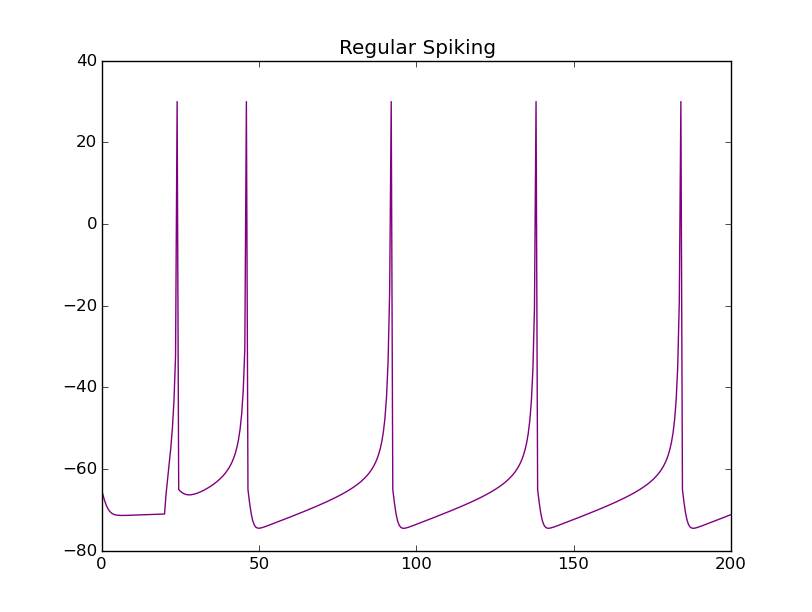
\includegraphics[scale=0.5]{figure_1}
\end{center}
\justify
\textsc{Regular Spiking}: le plus typique dans le cortex. Se présente par quelques décharges séparées par des courts intervalles de temps, et par la suite les décharges sont séparées par des périodes de plus en plus longs jusqu'à converger vers une certaine période.

\begin{center}
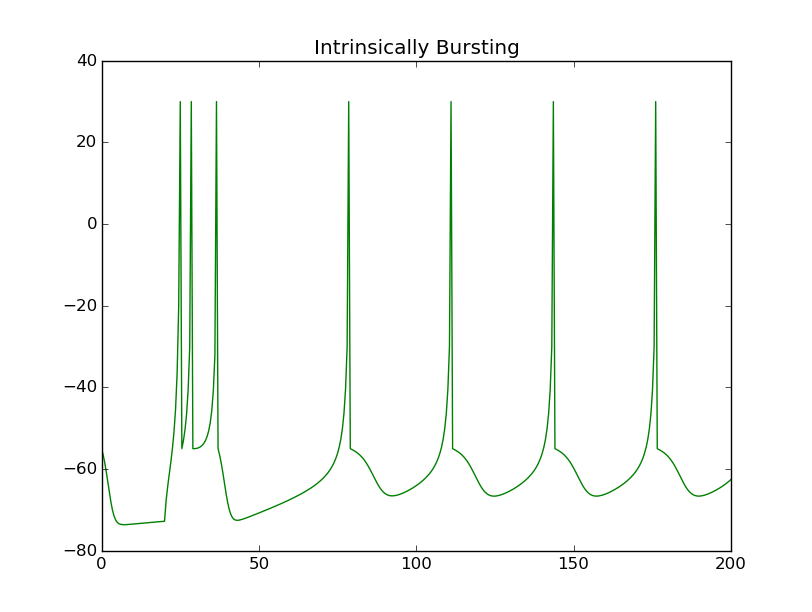
\includegraphics[scale=0.5]{figure_2}
\end{center}
\justify
\textsc{Intrisically Bursting:} Une bouffée, qui est ensuite suivie de décharges répétitives simples.

\begin{center}
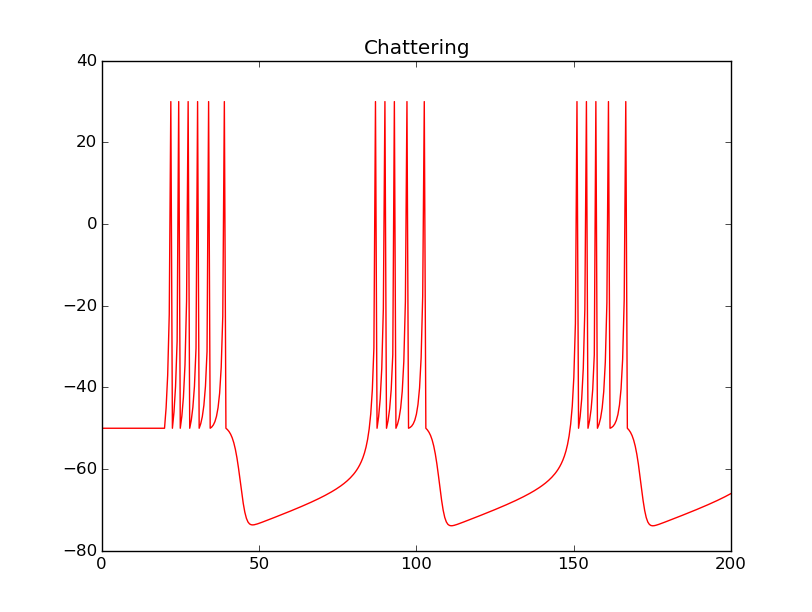
\includegraphics[scale=0.5]{figure_3}
\end{center}
\justify
\textsc{Chattering:} Une suite de bouffées régulièrement espacées dans le temps.
\justify
\textbf{- Neurones inhibiteurs: }
\justify
\begin{center}
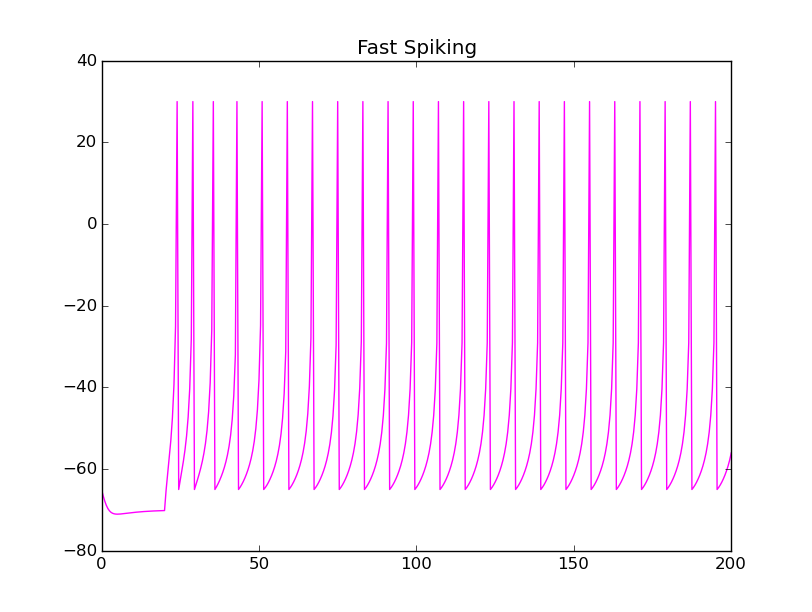
\includegraphics[scale=0.5]{figure_4}
\end{center}
\justify
\textsc{Fast Spiking:} Des décharges \`a très haute fréquence.

\begin{center}
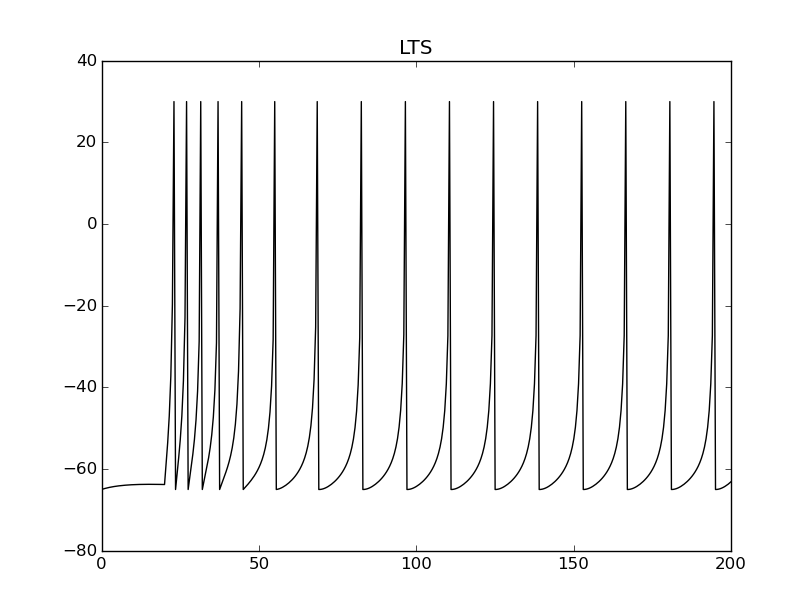
\includegraphics[scale=0.5]{figure_8}
\end{center}
\textsc{Low-threshold spiking:} Haute fréquence qui ensuite diminue légèrement pour atteindre une fréquence régulière.
\justify
\textbf{- Neurones thalamo-corticaux (TC)}: Il y a deux motifs de décharge selon le type de stimulation.
S’ils étaient au repos et qu’on les dépolarise, alors il y a quelques décharges séparées par de courts intervalles de temps, puis les intervalles de temps augmentent (1).
\begin{center}
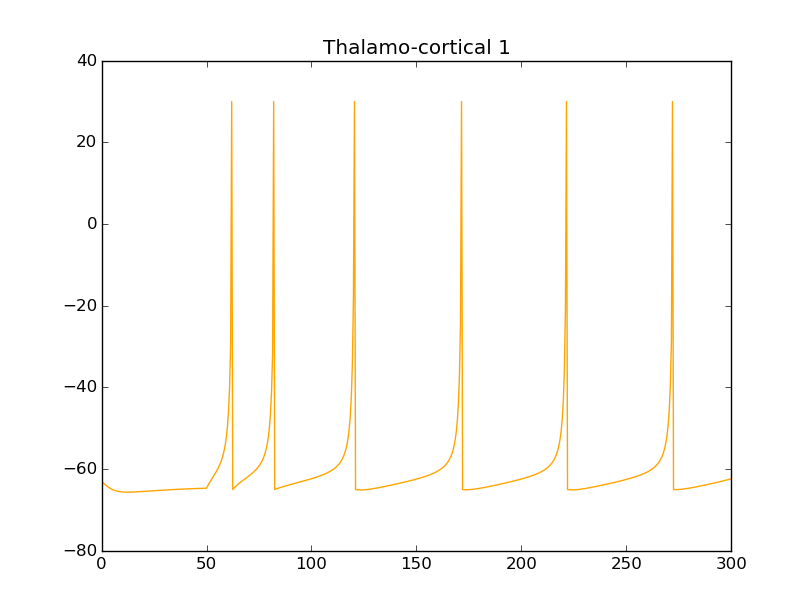
\includegraphics[scale=0.5]{figure_5}
\end{center}
\justify
S’ils reçoivent un courant négatif (pendant un certain temps), on observe une bouffée de décharges lorsque l’on on cesse la transmission (2).
\begin{center}
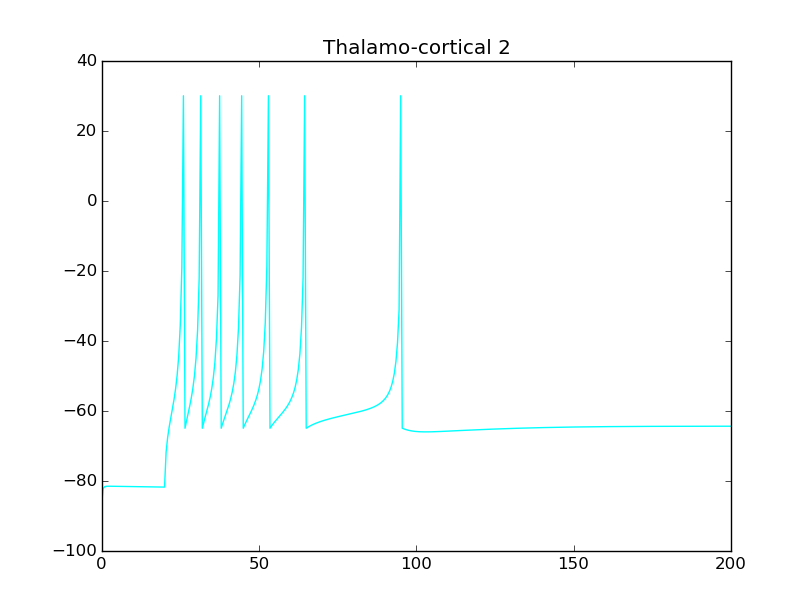
\includegraphics[scale=0.5]{figure_6}
\end{center}
\justify
Et finalement,
\begin{center}
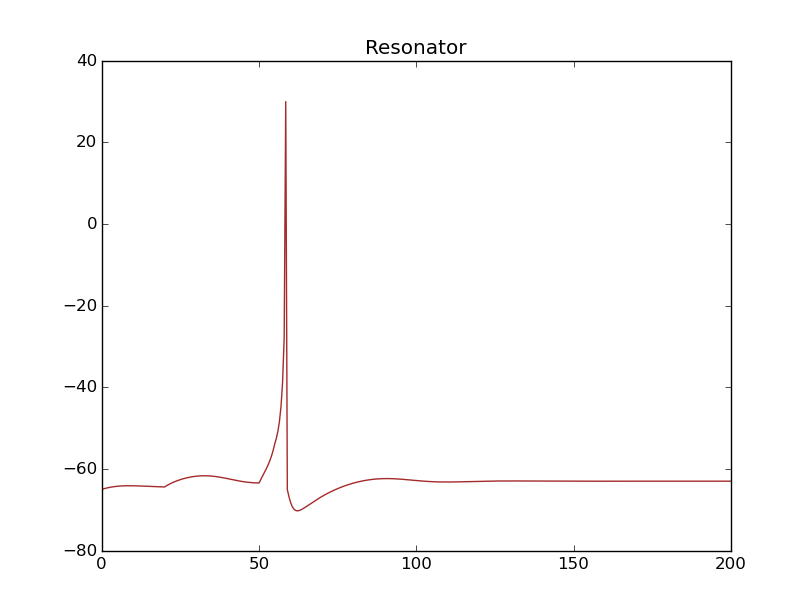
\includegraphics[scale=0.5]{figure_7}
\end{center}
\justify
\textsc{Resonator:} Si on stimule légèrement, on observe des oscillations très aplaties (de très faible amplitude), et si on augmente la stimulation ponctuellement, le neurone décharge régulièrement.
\justify
Le code \texttt{python} ci-dessous est une traduction "directe" du code \texttt{MATLAB} donn\'e par Izhikevich. Il simule un réseau de 1000 neurones en temps r\'eel.
\begin{python}
import numpy as np
import pylab as py
import matplotlib.pyplot as plot

__author__ = "Borjan Geshkovski & Charlotte Rodriguez"
__usage__ = "CC Neurosciences Computationelles"

Ne = 800
Ni = 200

re = py.rand(Ne)
ri = py.rand(Ni)

a = np.r_[0.02*np.ones(Ne), 0.02+0.08*ri]
b = np.r_[0.2*np.ones(Ne), 0.25-0.05*ri]
c = np.r_[-65+15*re**2, -65*np.ones(Ni)]
d = np.r_[8-6*re**2, 2*np.ones(Ni)]
S = np.c_[0.5*py.rand(Ne+Ni, Ne), -py.rand(Ne+Ni, Ni)]

v = -65*np.ones(Ne+Ni)			#Initial values of v.
u = b*v 						#Initial values of u.
firings = np.zeros((0,2))

for t in range(1000): 			#Stimulation of 1000 ms
	I = np.r_[5*py.randn(Ne), 2*py.randn(Ni)] #Thalamic input
	fired = py.find(v>=30) 					  #Indices of spikes
	if len(fired) != 0:
		firings = np.vstack((firings, np.c_[t+0*fired, fired]))
		v[fired] = c[fired]
		u[fired] = u[fired] + d[fired]
		I = I + S[:, fired].sum(1)
	v = v+0.5*(0.04*v**2+5*v+140-u+I)
	v = v+0.5*(0.04*v**2+5*v+140-u+I)
	u = u+a*(b*v-u)

plot.plot(firings[:, 0], firings[:, 1],  ".")
plot.title("Izhikevich's simple neuron network model")
plot.show()
\end{python}
\justify
On observe le résultat sur la figure ci-dessous.

\begin{center}
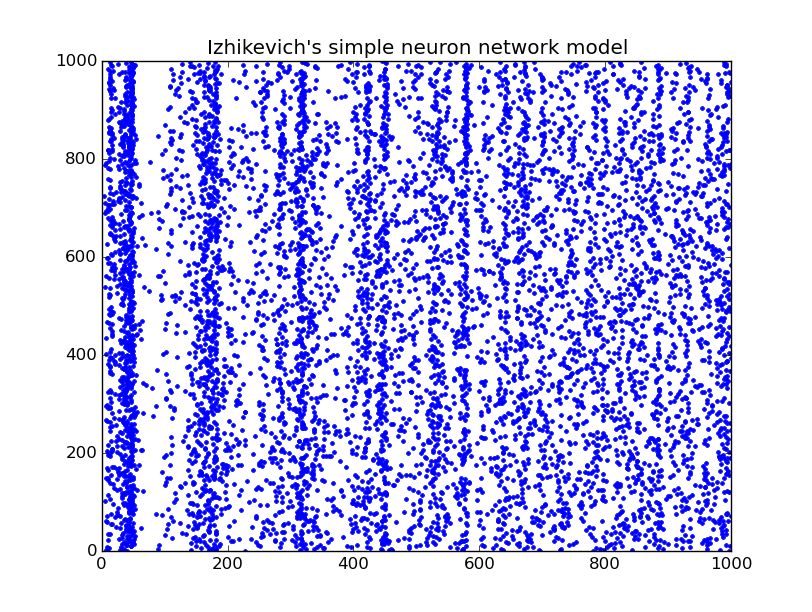
\includegraphics[scale=0.5]{figure_10}
\end{center}
\justify
\textsc{Pulse-Coupled Neural Network :} Ceci est une impl\'ementation du modèle d'Izhikevich dans le but de construire un réseau de "spiking neurons", qui semble capable d'exhiber une dynamique similaire \`a celle du cortex mammifère. Ce modèle restant très simpliste, permet une simulation d'un réseau de dix milles neurones en temps r\'eel.
\end{document}

		   


	


